\documentclass[11pt]{article}

\usepackage[margin=1in]{geometry}
\usepackage[T1]{fontenc}
\usepackage[utf8]{inputenc}
\usepackage{newtxtext,newtxmath}
\usepackage{microtype}
\usepackage{booktabs}
\usepackage{tabularx}
\usepackage{array}
\usepackage{footmisc}
\usepackage{titling}
\usepackage{amsmath}
\usepackage{xcolor}
\usepackage{abstract}
\usepackage{caption}
\usepackage{hyperref}
\usepackage{fontawesome5}
\usepackage[numbers,sort&compress]{natbib}
\usepackage{titlesec}
\usepackage{titling}
\usepackage{placeins}
\usepackage{graphicx}
\usepackage{xurl}
\usepackage{verbatim}
\usepackage{xspace}
\usepackage{pifont}
\graphicspath{{figures/}}

\hypersetup{
  colorlinks=true,
  linkcolor=blue!60!black,
  citecolor=blue!60!black,
  urlcolor=blue!60!black
}

\newcommand{\benchmarkname}{GameEngineBench\xspace}
\newcommand{\cmark}{\ding{51}}
\newcommand{\xmark}{\ding{55}}
\newcommand{\added}[1]{#1}
\newcommand{\addedtag}{}
\newcommand{\paperline}{\noindent\color{black!35}\rule{\columnwidth}{0.6pt}}

\setlength{\droptitle}{-1.2cm}
\setlength{\parindent}{0pt}
\setlength{\parskip}{0.6em}
\renewcommand{\abstractname}{Abstract}
\setlength{\absleftindent}{0pt}
\setlength{\absrightindent}{0pt}
\renewenvironment{abstract}
  {\par\noindent{\Large\bfseries\abstractname}\par\vspace{0.4em}\noindent}
  {\par\vspace{0.6em}}
\setlength{\abstitleskip}{-0.4em}
\captionsetup{
  font=small,
  labelfont=bf,
  labelsep=period,
  skip=4pt
}

\titleformat{\section}
  {\Large\bfseries}
  {\thesection}
  {0.6em}
  {}
\titlespacing*{\section}{0pt}{1.1em plus 0.2em minus 0.1em}{0.5em}

\pretitle{\par\raggedright\LARGE\bfseries}
\posttitle{\par\vspace{0.3em}\paperline\vspace{0.6em}}
\preauthor{\par\raggedright\normalsize}
\postauthor{\par}
\predate{}
\postdate{}

\title{\benchmarkname: Evaluating Coding Agents on Real C++ Runtime Environments}
\author{
  Brian La, Sejoon Chang, Ben Kim \\
  {\small Nitrode}\\[1em]
  Junyoung Bae \\
  {\small Nexon Intelligence Labs}\\[1em]
  Aamish Ahmad Beg$^{1}$, Sei Chang$^{2}$, Gonzalo Gonzalez-Pumariega$^{3}$\\
  {\small $^{1}$Dartmouth University $^{2}$Columbia University $^{3}$Cornell University}
}
\date{}

\begin{document}
\maketitle
\vspace*{-2em}
\renewcommand{\thefootnote}{\fnsymbol{footnote}}
\footnotetext[1]{The views and opinions expressed in this paper are those of the authors and do not necessarily reflect the official policy or position of their respective employers or affiliated institutions.}
\renewcommand{\thefootnote}{\arabic{footnote}}

\begin{flushleft}
\small
\faIcon{envelope}~~\href{mailto:research@nitrode.com}{\texttt{research@nitrode.com}}
\hspace{1em}
\faIcon{github}~~\href{https://github.com/Nitrode-Research/GameEngineBench}{\texttt{https://github.com/Nitrode-Research/GameEngineBench}}
\end{flushleft}

\begin{abstract}Game engines provide real-time simulation, rendering, physics, interaction, networking, and asset pipelines, making them valuable not only for games but also for 3D applications in healthcare, robotics, architecture, manufacturing, and related domains. Because game development is where these systems are most mature and publicly available, it offers a practical testbed for evaluating coding agents that must modify C++ code within stateful, interactive, real-time systems. We present \benchmarkname, a benchmark for evaluating coding agents on scoped C++ implementation tasks inside Unreal Engine 5 projects, built from nine real-world game repositories. The evaluation set consists of 110 tasks spanning gameplay mechanics, multiplayer behavior, AI and world orchestration, animation and movement, UI and session code, loading behavior, online-service integration, persistence, data serialization, XR behavior, and rendering-oriented plugins. These tasks require models to make native C++ changes that compile and satisfy behavioral tests within executable Unreal Engine projects. Across twelve evaluated configurations, the strongest model reaches 55.5\% pass@1, while 31 tasks remain unsolved by every configuration. Our results demonstrate that frontier coding agents continue to struggle with deeply integrated C++ development for real-time interactive software, highlighting game-engine benchmarks as a valuable complement to existing software engineering evaluations.
\end{abstract}

\FloatBarrier
\section{Introduction}
Coding agents are increasingly evaluated on realistic software engineering tasks, including long-horizon repository work and production-quality code review. However, existing benchmarks still largely focus on general-purpose software engineering. They do not directly measure whether generated C++ code can integrate with a running game engine, where correctness depends not only on language semantics but also on networking, object lifecycles, engine callbacks, assets, and interactions with existing gameplay systems. A patch may compile and appear plausible yet still fail because it updates only the local state, misses an object-lifecycle transition, or breaks an interaction with another engine system.

This setting extends beyond entertainment software. Modern game engines provide real-time simulation, rendering, physics, interaction, networking, and asset pipelines that are widely used in simulation, digital twins, XR, robotics prototyping, virtual production, and interactive training. Engine-based game development is a practical source of benchmark tasks for this broader class of software because game repositories are mature, executable, stateful, and often publicly available.

Evaluating game-engine tasks is challenging due to models needing to satisfy both C++ compilation and engine runtime behavioral requirements. Even a small implementation change may need to execute on the authoritative server, synchronize state across clients, update UI only for the local player, and correctly manage when actors are destroyed or reused. These behavioral requirements are simple to describe at a high level but hard to verify completely: a test suite can only run selected scenarios, while a truly correct Unreal implementation must satisfy behavior across connected systems, such as gameplay logic, replicated state, UI updates, and cleanup behavior.

Existing coding benchmarks capture important aspects of agent capability, including isolated function synthesis, issue resolution in software repositories, long-horizon codebase tasks, and multimodal game construction. However, they do not directly evaluate scoped native C++ edits inside functioning game-engine projects, where correctness depends on engine execution, networking behavior, object lifecycles, subsystem initialization, and integration with existing gameplay code. \benchmarkname addresses this gap using Unreal Engine projects as an executable testbed.

\benchmarkname contains 110 tasks drawn from nine publicly available Unreal Engine repositories. Each task gives the model a buildable start state, scoped editable C++ files, and a behavior specification. After the model finishes, tests are injected and executed through Unreal's Play-in-Editor automation, and judge auditing determines whether the implementation satisfies the requested behavior rather than merely matching a reference solution. Across 12 evaluated configurations, the strongest model reaches 55.5\% pass@1, while 31 tasks remain unsolved by every configuration. Many failed runs still recover substantial partial behavior, but the failures cluster around recurring runtime and integration patterns, including authority mistakes, state-synchronization errors, object-lifecycle bugs, initialization errors, and incomplete integration with surrounding game systems.

We make three contributions. First, we introduce a 110-task benchmark for evaluating C++ changes that require integration into functioning Unreal Engine projects. Models edit only native source files, although the projects themselves may include non-code assets required during execution.\footnote{Some source projects use non-code assets during execution, but benchmarked edits are restricted to native C++ files.} Second, we define an evaluation protocol that combines scoped file edits, runtime tests, and judge auditing to score behavioral correctness rather than reference similarity. Third, we analyze the failure modes of current coding agents, showing that low pass@1 reflects structured runtime and integration failures rather than superficial syntax errors or compilation failures alone. By grounding coding tasks in executable game projects, \benchmarkname provides a concrete measure of coding-agent capability on game-engine development.

% Trained on the TF Atlas scRNA-seq data that capture the differentiation pathways of cells perturbed by overexpression of more than a thousand TFs, PerturbODE enables scalable and interpretable discovery of the gene dependencies that drive cellular differentiation. 

\FloatBarrier
\section{Related Work}

\textbf{Software Engineering Benchmarks}. Software engineering has become a central domain for evaluating LLM-based coding agents. Earlier code-generation benchmarks such as HumanEval and MBPP measure isolated function synthesis \citep{chen2021evaluating,austin2021programsynthesis}. SWE-bench evaluates whether models can resolve real GitHub issues in conventional software repositories \citep{jimenez2023swebench}; SWE-bench-Live and SWE-rebench emphasize freshness, continuous task collection, and contamination-resistant evaluation \citep{zhang2025swebenchlive,badertdinov2025swerebench}; Terminal-Bench evaluates agents on realistic command-line tasks that require operating inside an execution environment \citep{merrill2026terminalbench}. These benchmarks establish bug fixing and environment-level execution as important alternatives to isolated coding problems. \benchmarkname targets a different part of the software-engineering spectrum by evaluating larger implementation tasks inside functioning runtime systems, using game projects as the concrete execution environment. Across the 110 evaluated tasks, reference solutions add a mean of 511 lines and a median of 362 lines within the editable source files, making the tasks larger than the SWE-bench Verified and SWE-bench Pro reference edits reported by DeepSWE \citep{huang2026deepswe}. This shifts the evaluation from localized bug repair toward implementing missing behavior inside an existing runtime system.

\textbf{Frontier Agent Benchmarks}. Recent agent benchmarks have shifted from step-by-step implementation specifications to realistic behavior-focused instructions that require deeper reasoning and understanding. DeepSWE evaluates frontier coding agents on original, long-horizon software engineering tasks with broad repository coverage and behavior-focused verifiers \citep{huang2026deepswe}. ProgramBench evaluates whether agents can rebuild complete software projects from documentation and executable behavior, showing that agents often produce codebases that behave partially correctly but diverge sharply from human-written implementations \citep{yang2026programbench}. FrontierCode shares the emphasis on realistic codebase tasks, but uses maintainer-authored tasks and rubric-based grading to shift the target from behavioral correctness alone toward mergeability, evaluating whether generated code would meet production codebase standards \citep{lu2026frontiercode}. \benchmarkname follows this direction while focusing on runtime-integrated C++ programming.

\textbf{Game Development Benchmarks}. GameDevBench establishes game development as a meaningful domain for agent evaluation with tasks derived from web and video tutorials, emphasizing multimodal game-development work such as visual scenes, shaders, sprites, and animations \citep{chi2026gamedevbench}. AutoUE studies automated 3D game generation in Unreal Engine through multi-agent systems and automated play-testing, but targets end-to-end game creation rather than constrained C++ changes inside existing projects \citep{yin2026autoue}. GameDevBench does not target multiplayer or server/client correctness, which are central sources of failure in networked game development. \benchmarkname instead evaluates native C++ changes inside existing Unreal projects. This focuses the benchmark on runtime-integrated programming, where code must work with existing gameplay logic, networking, and engine architecture.

\begin{table}[t]
\centering
\scriptsize
\setlength{\tabcolsep}{3pt}
\resizebox{\linewidth}{!}{%
\begin{tabular}{@{}lcccccccr@{}}
\toprule
\textbf{Benchmark} & \textbf{Existing repo} & \textbf{Patch/edit task} & \textbf{Full project gen.} & \textbf{Game engine} & \textbf{Native C++} & \textbf{Server/client} & \textbf{Judge/rubric audit} & \textbf{Tasks} \\
\midrule
SWE-bench \citep{jimenez2023swebench} & \cmark & \cmark & \xmark & \xmark & \xmark & \xmark & \xmark & 2,294 \\
DeepSWE \citep{huang2026deepswe} & \cmark & \cmark & \xmark & \xmark & \xmark & \xmark & \cmark & 113 \\
FrontierCode \citep{lu2026frontiercode} & \cmark & \cmark & \xmark & \xmark & \xmark & \xmark & \cmark & 150 \\
ProgramBench \citep{yang2026programbench} & \xmark & \xmark & \cmark & \xmark & \xmark & \xmark & \xmark & 200 \\
GameDevBench \citep{chi2026gamedevbench} & \xmark & \cmark & \xmark & \cmark & \xmark & \xmark & \xmark & 333 \\
AutoUE \citep{yin2026autoue} & \xmark & \xmark & \cmark & \cmark & \xmark & \xmark & \xmark & -- \\
\benchmarkname & \cmark & \cmark & \xmark & \cmark & \cmark & \cmark & \cmark & 110 \\
\bottomrule
\end{tabular}}
\caption{High-level comparison with related coding-agent and game-development benchmarks. Checkmarks denote properties that are central to the benchmark design rather than incidental capabilities. \benchmarkname uniquely combines existing game-engine repositories, scoped native C++ edits, server/client correctness, and LLM-reviewed runtime behavior.}
\label{tab:benchmark-comparison}
\end{table}
\textbf{Game-Engine Runtime Behaviors}. We define four runtime behaviors that are fundamental to correctly solving Unreal Engine programming tasks. \emph{Multiplayer authority} requires authoritative gameplay decisions to run on the server rather than on individual clients; this follows the client/server model used by Unreal networking \citep{epic2026networking}. \emph{Replication} is Unreal's mechanism for synchronizing gameplay state and procedure calls between server and clients; property replication sends server-side updates to connected clients, which then apply those values to their local actor instances \citep{epic2026networking,epic2026replicateactorproperties}. \emph{Object lifecycle} refers to the sequence of actor and object events around spawning, initialization, gameplay start, teardown, destruction, and garbage collection \citep{epic2026actorlifecycle}. \emph{Subsystem architecture} refers to Unreal-managed systems such as game-instance, world, and local-player subsystems that the engine creates, initializes, and exposes to gameplay code \citep{epic2026subsystems}. Correct implementations often depend on coordinating these behaviors to produce a correct solution to a development task. The emphasis on cross-system behavior is consistent with prior work showing that game-engine subsystems are tightly coupled and hard to understand in isolation \citep{ullmann2023visualising}. A compilable solution can still fail if it runs on the wrong machine, updates only local state, cleans up too late, or registers a component after another system expects it to exist.

\begin{figure}[t]
\centering
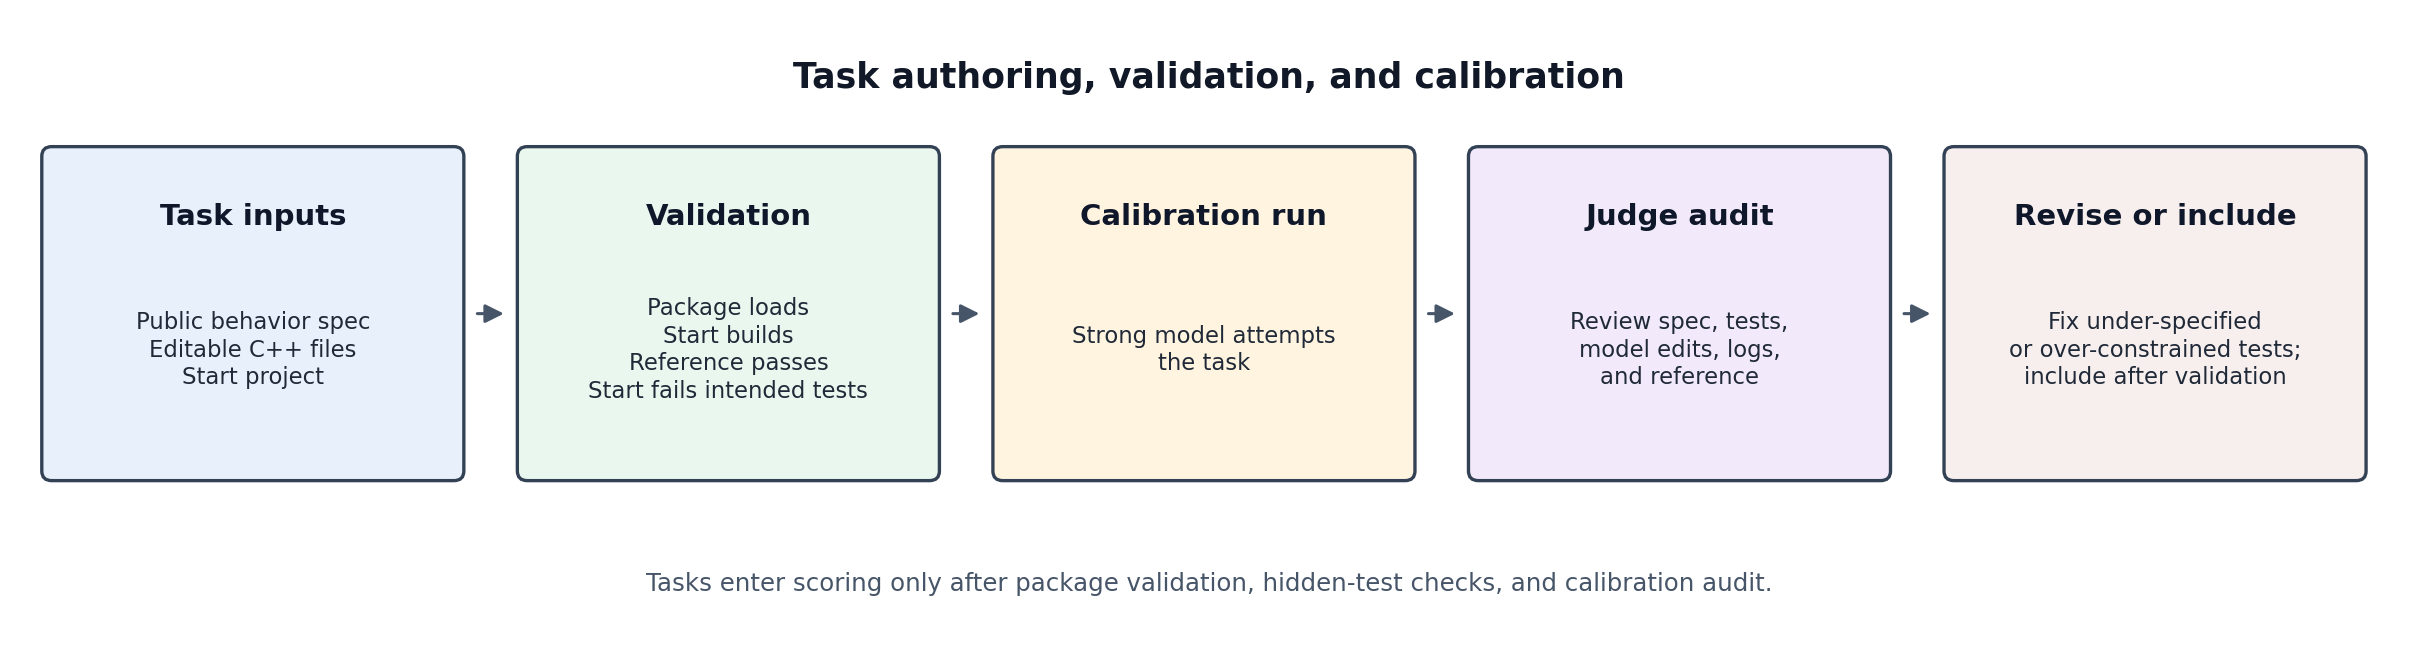
\includegraphics[width=0.95\linewidth]{task_authoring.png}
\caption{Task authoring, test validation, LLM-as-a-Judge review, and task calibration process.}
\label{fig:task-authoring}
\end{figure}

\FloatBarrier
\section{Benchmark Design}

Every task provides the model with a buildable starting state, a list of editable C++ files, and a public set of text instructions that define observable task-specific behavior. The test suite is withheld from the solver workspace and injected only after the model completes its implementation, preventing leakage of evaluation logic during the solve phase.

Before a task is included in the benchmark, we use a multi-step authoring process with two distinct checks. \emph{Test validation} checks that the task package loads, the start project builds, the reference solution passes the tests, and the starting state fails those tests on the intended missing behaviors. \emph{LLM-as-a-Judge review} runs a strong coding model on the task and asks an LLM judge to review the saved result against the public behavior specification, test outcomes, model edits, and reference solution. This review identifies tests that are under-specified, too narrow, or over-constrained relative to the requested behavior. When issues are found, we revise the task or test suite and repeat the validation process. We refer to this iterative pre-release workflow of task validation, judge review, task refinement, and revalidation as \emph{task calibration}. Figure~\ref{fig:task-authoring} summarizes the process.

\FloatBarrier
\section{Current C++ Task Set}
The current evaluated task set consists of 110 active tasks and is sourced from nine Unreal projects. The tasks focus on gameplay and systems programming within existing codebases, spanning gameplay mechanics, multiplayer behavior, AI and world orchestration, animation and character systems, UI and player-session systems, subsystem and plugin integration, runtime object management, data/configuration logic, movement systems, XR behavior, and rendering-oriented plugin code. The benchmark is not intended to cover every aspect of C++ game development; coverage is intentionally lighter for domains such as audio, performance, platform support, security, and tooling.

\begin{figure}[t]
\centering
\includegraphics[width=.6\linewidth]{task_gallery.png}
\caption{Example tasks from GameEngineBench. Screenshots are taken from reference solutions to illustrate the gameplay and engine-system behaviors evaluated by the benchmark.}
\label{fig:task-gallery}
\end{figure}
  
The tasks are sourced from nine open-source Unreal projects: HordeTemplateV2Native, ActionRoguelike, Bomber, TargetVector, GASShooter, Eternal Crusade Resurrection, LASAA, PBMovementBench, and NanoGSBench. We selected these repositories to maximize diversity in project context. Because each task remains embedded within its original codebase, the model must work with existing C++ code, engine callbacks, networking setup, and gameplay architecture instead of solving isolated programming problems. Figure~\ref{fig:task-area-distribution} summarizes the distribution of tasks across game-development areas. Two sample tasks are described in Appendix~\ref{app:sample-tasks}.

\begin{figure}[t]
\centering
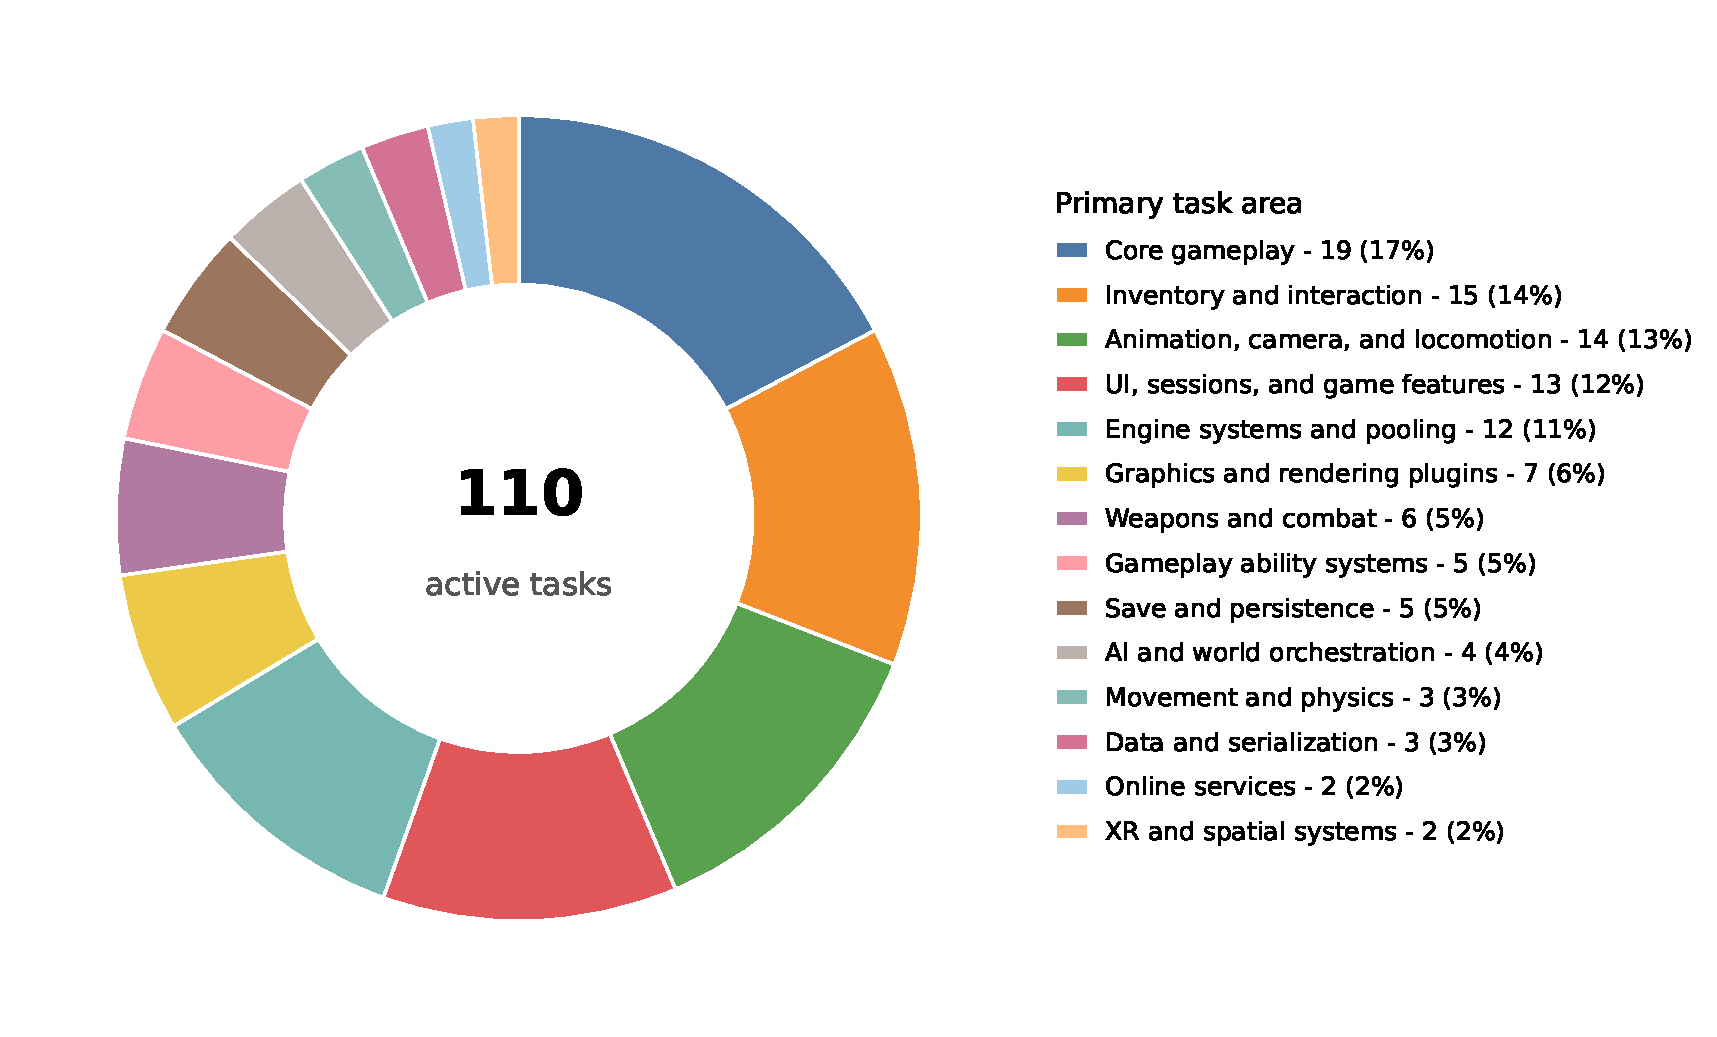
\includegraphics[width=0.7\linewidth]{task_area_distribution.pdf}
\caption{Primary game-development areas covered by the current task set. Categories are assigned once per task for readability; many tasks also exercise cross-cutting runtime requirements such as authority, state synchronization, object lifecycle handling, and subsystem initialization.}
\label{fig:task-area-distribution}
\end{figure}

\FloatBarrier
\section{Evaluation Protocol}
The primary evaluation metric used in this work is \emph{pass@1}, defined as the fraction of tasks solved by a single model attempt. A run is counted as successful when the LLM judge determines that the generated implementation satisfies the requested behavior. This LLM-judged definition is necessary because the tasks often span several engine systems, making it impractical for any test suite to capture every valid implementation and interaction path.

The LLM review follows the LLM-as-a-Judge paradigm. It receives the behavioral specification, test source, execution results and assertion failures, model's code edits, and reference solution, then determines whether the implementation satisfies the intended task behavior \citep{zheng2023judging}. The LLM's role is not to measure similarity to the reference solution, but to assess behavioral correctness and determine whether the test results accurately reflect that correctness. To mitigate self-judging bias, the evaluation protocol supports cross-family judging whenever multiple model families are available.

Each run is executed by the benchmark CLI in an isolated temporary workspace copied from the task's public \texttt{start/} state. The CLI invokes each agent through its public command-line wrapper with the same task payload: the behavior specification, the list of editable files, and the requirement that the modified project must compile successfully. Public CLI wrappers provide a reproducible interface while preserving each agent's standard tool-use behavior. After the solve phase, tests are injected and executed through Unreal's automation framework in Play-in-Editor (PIE) listen-server mode \citep{epic2026piemultiplayer}. The benchmark preserves the resulting workspace, logs, and judge output for auditing. Staging the evaluation process reduces leakage, preserves reproducibility, and maintains a clear distinction between the public task specification, tests, and judge review.

\begin{table}[t]
\centering
\small
\setlength{\parindent}{0pt}
\setlength{\parskip}{0.6em}
\setlength{\tabcolsep}{5pt}
\begin{tabular}{@{}p{0.30\textwidth}p{0.60\textwidth}@{}}
\toprule
\textbf{Execution detail} & \textbf{Current setup} \\
\midrule
Evaluated model setups & \texttt{gpt-5.5} (\texttt{xhigh}/\texttt{high}/\texttt{medium}) + \texttt{codex}; \texttt{claude-fable-5} (\texttt{max}), \texttt{claude-opus-4-8} (\texttt{max}/\texttt{high}), \texttt{claude-opus-4-7} (\texttt{high}), and \texttt{claude-sonnet-4-6} (\texttt{high}) + \texttt{claude-code}; \texttt{Gemini 3.1 Pro} + Antigravity CLI; \texttt{DeepSeek 4 Pro} and \texttt{Qwen 3.7 Plus} + \texttt{qwen-code}; \texttt{Kimi for Coding} + \texttt{kimi-code} \\
Task mode & Unreal automation in PIE listen-server mode \\
Solve attempts & One per task/model pair; no retries or majority vote \\
Reasoning effort & Explicit where supported by the wrapper: \texttt{gpt-5.5} uses \texttt{xhigh}/\texttt{high}/\texttt{medium}; Claude configurations use \texttt{max}/\texttt{high}; other wrappers use their configured default. \\
Timeouts & Solver: 3600 s; compile and test: 600 s each \\
Scoring & pass@1 \\
\bottomrule
\end{tabular}
\caption{Execution setup for the current evaluated task set.}
\label{tab:execution-setup}
\end{table}

\FloatBarrier
\section{Results}
We report pass@1 as the primary evaluation metric. The results show that the benchmark is not saturated by current coding agents. The strongest evaluated configuration reaches 55.5\% pass@1, while several other frontier configurations remain far below that level. The results also show that model capability is not strictly ordered: a configuration with higher overall pass@1 can still miss tasks solved by a lower-scoring configuration. In addition, 31 tasks are not solved by any evaluated configuration.
\subsection{Success Rates}
Figure~\ref{fig:main-success-rate} provides the main model comparison. The best evaluated configuration is \texttt{claude-fable-5} with \texttt{max} reasoning effort at 55.5\% pass@1. The next strongest configuration is \texttt{GPT-5.5} with \texttt{xhigh} reasoning effort at 29.1\%, followed by \texttt{claude-opus-4-8} with \texttt{max} effort at 23.6\% and \texttt{Gemini 3.1 Pro} at 18.2\%.

\begin{figure}[t]
\centering
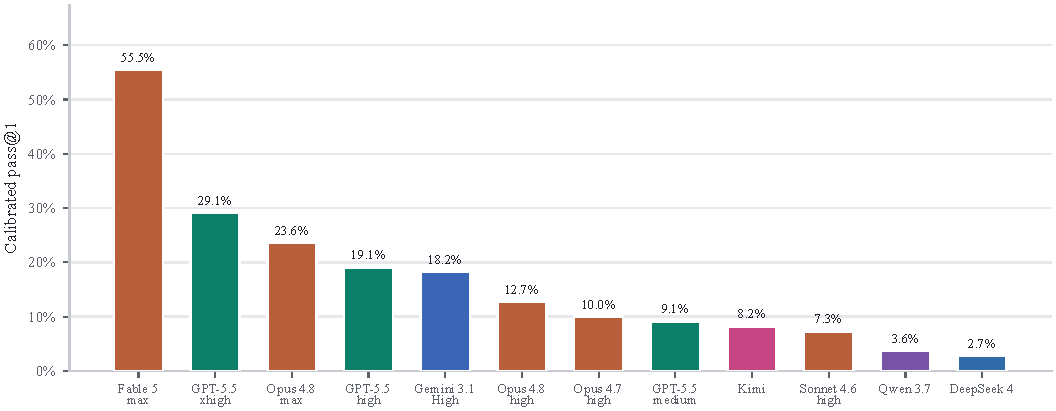
\includegraphics[width=0.96\linewidth]{21_calibrated_success_rate.pdf}
\caption{Success rate by model configuration over the active 110-task set. Each label includes the model and reasoning effort where applicable.}
\label{fig:main-success-rate}
\end{figure}

The gap between the strongest configuration and the rest of the evaluated agents is large. This suggests that the benchmark is sensitive to meaningful differences between model--harness setups rather than assigning similar scores to all frontier systems. At the same time, the strongest configuration still leaves nearly half of the benchmark unsolved. The task set is therefore not saturated: even the best current agent does not reliably solve C++ systems work inside existing Unreal projects.

The \texttt{GPT-5.5} reasoning-effort sweep gives a second view of this difficulty. Increasing reasoning effort from \texttt{medium} to \texttt{high} to \texttt{xhigh} raises pass@1 from 9.1\% to 19.1\% to 29.1\%. Additional reasoning helps substantially, but it does not close the gap to the strongest configuration and does not make the benchmark easy. This indicates that some failures are recoverable through more search and deliberation, while many still require better handling of runtime behavior and project integration.

% \subsection{Partial Progress Is Much Higher Than Full-Task Success}
% The lower-scoring configurations are still often related to the requested behavior. Several configurations satisfy well over half of the individually judged requirements while solving far fewer complete tasks. For example, \texttt{GPT-5.5} at \texttt{xhigh} reaches 29.1\% pass@1 but 80.4\% mean requirement satisfaction, and \texttt{claude-opus-4-8} at \texttt{max} reaches 23.6\% pass@1 but 77.9\% mean requirement satisfaction. \texttt{claude-fable-5} is the strongest configuration on both measures, reaching 55.5\% pass@1 and 91.1\% mean requirement satisfaction.


% This gap is important for interpreting the benchmark. Unreal tasks often require several behaviors to work together: code can satisfy the obvious local pieces, compile successfully, and still fail because one runtime dependency is wrong. A client may lack the state needed by a UI update, a pooled actor may retain stale state, or a subsystem may become available after another component expects it to exist. The benchmark therefore distinguishes partial implementation progress from complete behavioral correctness.

\subsection{Efficiency Tradeoffs}
% The clearest within-model trend is the \texttt{GPT-5.5} reasoning-effort sweep. Moving from \texttt{medium} to \texttt{high} to \texttt{xhigh} increases pass@1 from 9.1\% to 19.1\% to 29.1\%. This is a large gain, but it is not a complete explanation of performance: the \texttt{xhigh} run also spends more time, cost, and output tokens, and it still leaves most tasks unsolved.

Appendix Figure~\ref{fig:efficiency-frontier-main} shows the resource tradeoffs behind the pass@1 ranking. \texttt{claude-fable-5} gives the strongest pass@1, while \texttt{GPT-5.5} at \texttt{xhigh} is faster and less expensive in this run. \texttt{Gemini 3.1 Pro} is faster and cheaper than both, but with lower pass@1. These tradeoffs must be considered because the best agent may not be the most practical agent in the workflow. Cheaper agents can properly solve simpler tasks and can be deployed more at scale effectively. The efficiency of these models should be considered in conjunction with the pass@1 leaderboard.

\subsection{Solved Sets Are Complementary}
The leaderboard does not imply a strict nesting of capabilities. Appendix Figure~\ref{fig:coverage-complementarity} shows that 79 tasks are solved by at least one configuration, while 31 tasks are not solved by any of the twelve configurations. Conversely, no task is solved by all configurations.

\FloatBarrier

The complementarity analysis reveals structure in model performance that is not visible from a single ranking. Some tasks are solved by only one or two configurations, indicating that changing models can recover specific behaviors. At the same time, the 31-task no-solve subset shows that model selection alone is insufficient to cover the benchmark. Overall, the current frontier is broad but incomplete: different agents succeed on different parts of the task set, while a substantial set of tasks remains unsolved across all evaluated configurations.

\subsection{Coverage Varies By Task Area}
The no-solve set is not uniformly distributed across task categories. Figure~\ref{fig:task-area-coverage} groups tasks by task area and stratifies tasks solved by at least one configuration from unsolved tasks. In this view, save and persistence have the largest unresolved share. Furthermore, weapons/combat, serialization, UI/game-feature work, AI/world orchestration, animation/locomotion, engine systems/pooling, core gameplay, rendering plugins, and inventory/interaction all retain at least one unsolved task.

\FloatBarrier

Tasks that remain unsolved for any configuration share a common failure mode: cross-system coordination. The SPUD persistence tasks require actor identity, destroyed actors, serialized properties, streaming levels, and save/load lifecycle code to remain consistent across sessions. Task \texttt{1} (Zombie System) requires AI control, round-state updates, server-authoritative damage, player-state rewards, replicated feedback, and spawn metadata to agree. Task \texttt{19} (Generated Map Orchestrator) requires generation, actor pooling, replication, and readiness signaling to stay synchronized. These tasks are difficult for agents because correctness requires coordination between several runtime systems, rather than the use of any single Unreal API call.

\subsection{Failure Mechanisms}

\begin{figure}[t]
\centering
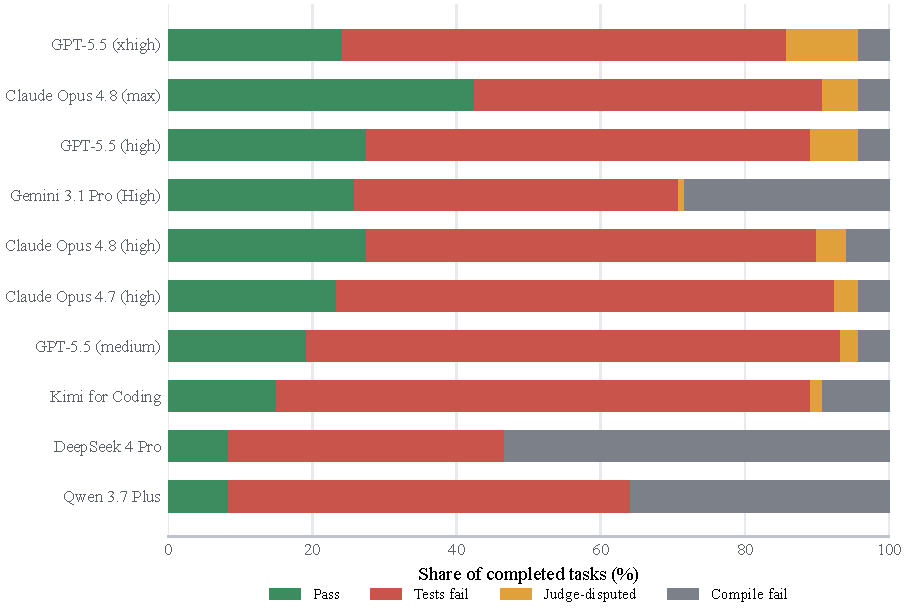
\includegraphics[width=0.78\linewidth]{11_failure_modes.pdf}
\caption{Outcome decomposition per configuration.}
\label{fig:failure-compile}
\end{figure}

We uncover failure mechanisms from model-level and task-level results that explain the task-coverage gap. Figure~\ref{fig:failure-compile} decomposes outcomes into passes, test failures, judge-disputed cases, and compile failures. The higher-performing wrappers usually reach compilation and execution; their remaining errors are mostly behavioral rather than purely syntactic.

For example, in active-item replication tasks, models occasionally add an \texttt{OnRep} hook but leave the client without the replicated source state needed to update visible UI. In player-controller and menu tasks, models can omit local-controller checks, allowing client-specific browsing or playback state to run on the wrong controller instance. In ability and action-system tasks, models often recover declarations but miss constructor defaults, activation timing, or teardown behavior. The generated output resembles plausible Unreal C++ code, but the runtime behavior is incomplete.

\FloatBarrier
\section{Limitations and Next Steps}
The current task set provides a strong foundation for evaluating model capabilities on Unreal C++ development. The tasks offer broad coverage of gameplay-facing C++ systems within existing projects, including combat, inventory, networking, actor lifecycle, player/session flows, subsystem integration, and data/configuration behavior. However, the task coverage does not extend to other important areas of C++ game engineering, such as audio, memory, performance, platform support, editor tools, build systems, and security-sensitive code.

The choice of source repositories also imposes an inherent ceiling on coverage. Open-source Unreal projects typically expose gameplay and framework code more readily than proprietary engine modifications, rendering work, platform integrations, performance infrastructure, or security-sensitive systems. As a result, the current evaluated set captures a substantial but incomplete slice of professional C++ game engineering.

The execution harness introduces an additional boundary. Running tasks through PIE listen-server automation is a practical way to test runtime behavior, authority, replication, and lifecycle correctness, but it does not fully reflect production environments that rely on dedicated server fleets, console hardware, performance profiling, large QA matrices, or long-running live operations. Moreover, test suites are inherently imperfect due to not capturing all valid implementations, making evaluation sensitive to both test design and judge calibration.

Future expansion could expand coverage in two directions. First, the benchmark should include more tasks that require coordination across multiple engine systems, which are common in game repositories but still remain difficult for frontier coding agents. Second, a separate expansion should incorporate underrepresented areas of C++ game development, such as audio, performance, editor tooling, build/platform code, and security-sensitive gameplay infrastructure. Together, these additions would improve representation while preserving the engine-integrated runtime challenges that define the benchmark.

We also identify two methodological extensions that strengthen evaluation reliability. First, because the evaluated models are run through different wrappers, the observed pass@1 differences partially reflect wrapper effects rather than pure model capability. Standardizing the execution wrapper will yield fairer comparisons. Second, LLM review can convert some test failures into valid solutions, showing that the tests do not always capture the full behavior space of these tasks. Improving test coverage and calibration would reduce reliance on judge intervention and produce a more direct execution signal.

\FloatBarrier
\section{Conclusion}
\benchmarkname marks a concrete step toward benchmark design for AI-assisted C++ programming. Rather than evaluating agents on narrowly specified instructions, our benchmark requires generated outputs to align with behavioral requirements at runtime, thereby testing whether models understand context and correctly integrate with the surrounding game system. The tasks are extracted from executable Unreal Engine repositories, enabling evaluation of production-like C++ runtime behaviors while leaving several areas of game development for future expansion. The 110-task set shows that frontier coding agents do not reliably integrate with gameplay-facing C++ systems easily, failing to replicate runtime behavior despite meeting syntax and compilation requirements. While the benchmark is specific to Unreal Engine, the observed performance gaps reflect broader challenges in engine- and framework-integrated software development, where generated code must operate within existing systems, respect execution constraints, and preserve behavior under realistic runtime conditions. As a result, \benchmarkname{} serves both as a focused benchmark for challenging C++ game development and as a foundation for more comprehensive evaluations of programming within game engines in future work.

\bibliographystyle{plainnat}
\bibliography{references}

\appendix
\section{Sample Tasks}
\label{app:sample-tasks}
Two examples illustrate the kinds of Unreal work included in the current evaluated task set. We choose these examples because both remain pass@1 failures for all evaluated configurations and expose different forms of engine-level coordination.

Task \texttt{1} (Zombie System) is a broad multiplayer gameplay task in HordeTemplate. It requires coordinated edits across eight source files so zombies spawn through the round system, update the alive-zombie counter, detect and pursue living players, stop acting after death, enforce melee range, award kill and headshot rewards, and expose attack/death feedback to clients. The task is difficult because correctness depends on several systems agreeing at once: AI control, game-mode round progression, player-state rewards, server-authoritative damage, replicated feedback, and spawn/patrol metadata.

Task \texttt{19} (Generated Map Orchestrator) is narrower in file count but still integration-heavy. It requires a generated map actor to populate a procedural grid at round start, reuse pooled actors across regenerations, send one ready signal after local generation completes, replicate map-size changes, and keep peers synchronized. This task is difficult because the implementation must coordinate generation, actor pooling, replication, editor preview behavior, and readiness signaling without firing too early, firing twice, or leaking actors across regenerations. Together, these examples show that the benchmark's hardest tasks are not defined only by edit size; they require consistent behavior across interacting Unreal systems.


\section{Supplemental Result Figures}
The main text uses the figures needed for the core findings. This appendix includes denser diagnostic views that support those findings without interrupting the Results narrative. These figures are intended as audit views: they expose alternative scoring lenses, task-level structure, metadata breakdowns, compiler behavior, and resource use behind the headline pass@1 table.

\begin{figure}[t]
\centering
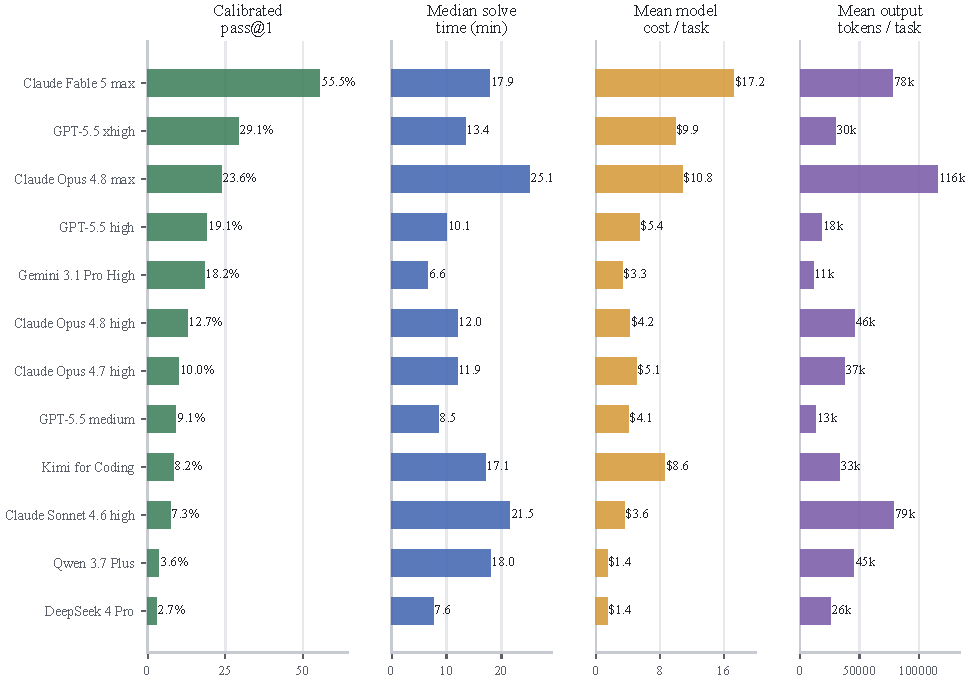
\includegraphics[width=0.95\linewidth]{18_efficiency_frontier.pdf}
\caption{Efficiency profile across evaluated configurations. Rows are sorted by pass@1 and compare success rate with median solve time, mean model cost, and mean output tokens per task.}
\label{fig:efficiency-frontier-main}
\end{figure}

\begin{figure}[!htbp]
\centering
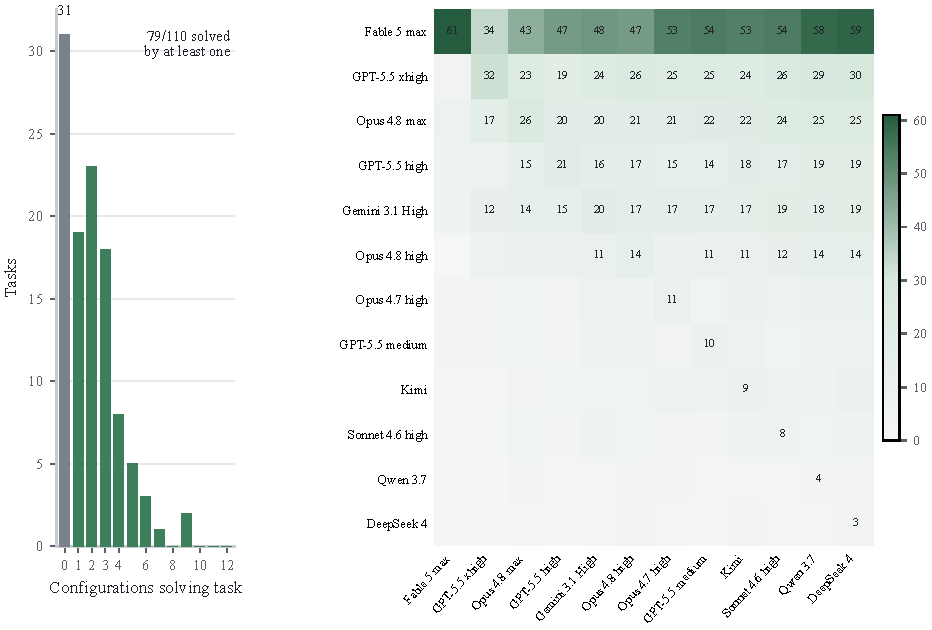
\includegraphics[width=0.96\linewidth]{28_calibrated_coverage_complementarity.pdf}
\caption{Task coverage and model complementarity. Left: how many configurations solve each task. Right: each off-diagonal entry counts tasks solved by the row configuration but missed by the column configuration; diagonal entries are own solved counts.}
\label{fig:coverage-complementarity}
\end{figure}

\begin{figure}[!htbp]
\centering
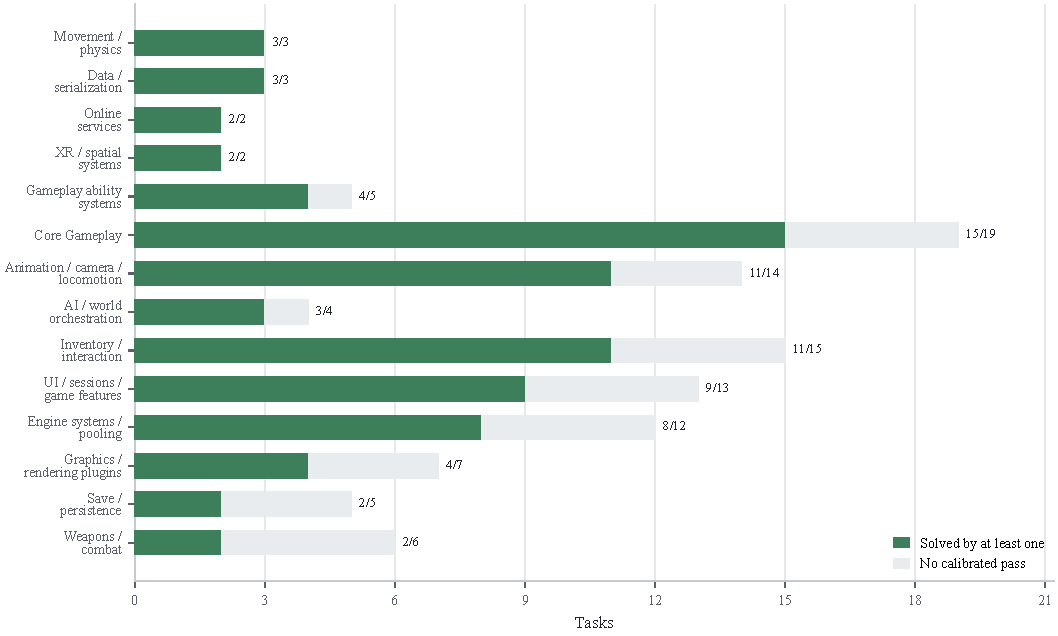
\includegraphics[width=0.88\linewidth]{27_task_area_coverage.pdf}
\caption{Task-area coverage under pass@1. Green segments count tasks solved by at least one evaluated configuration; gray segments count tasks with no successful runs. Labels at the end of each bar show the number of solved tasks over the total number of tasks in each area.}
\label{fig:task-area-coverage}
\end{figure}

\begin{figure}[t]
\centering
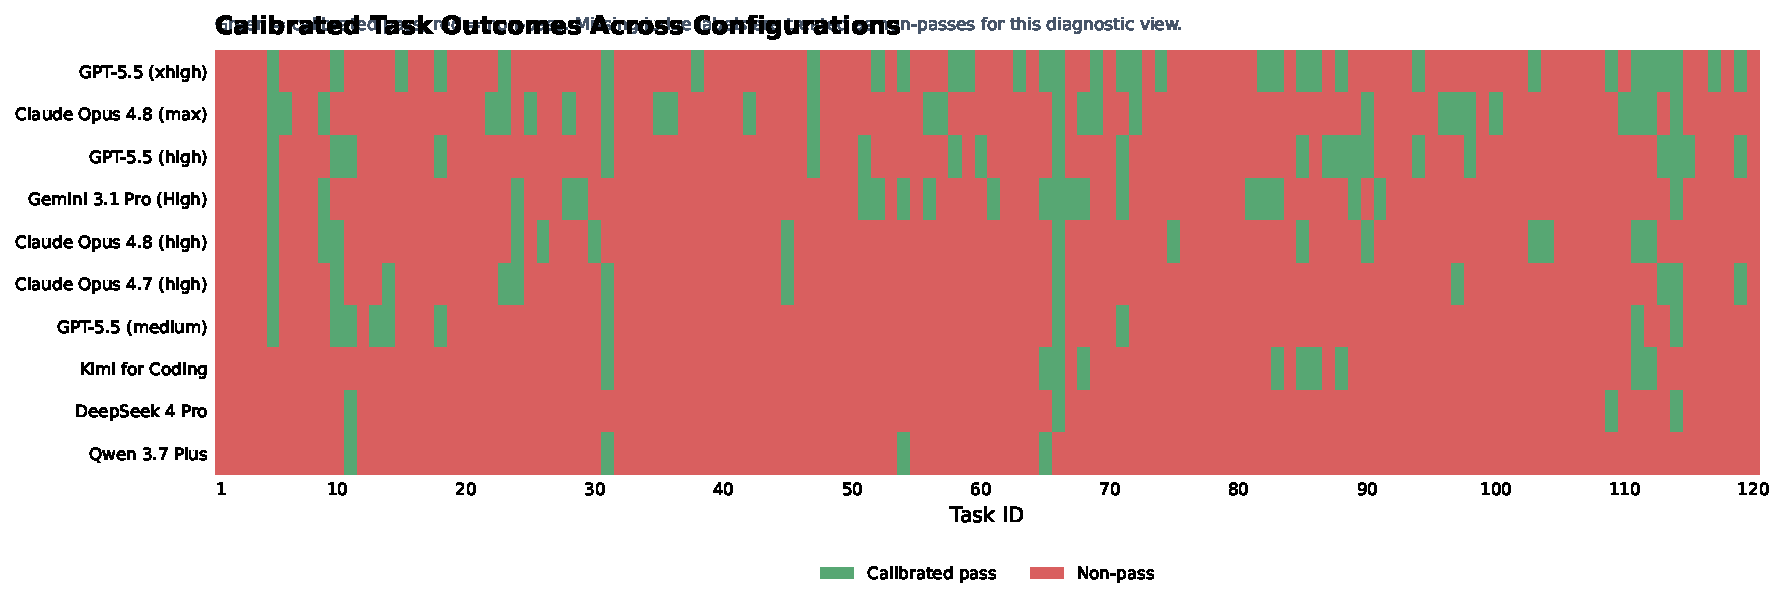
\includegraphics[width=0.92\linewidth]{24_calibrated_task_outcome_matrix.pdf}
\caption{Per-task outcome matrix over the active 110-task set. Green cells are passes; red cells are non-passes. This dense view supports the capability-frontier analysis in the main text.}
\label{fig:appendix-task-matrix}
\end{figure}

Figure~\ref{fig:appendix-task-matrix} preserves the task-level detail that is hidden by aggregate pass@1. Rows show model configurations and columns show tasks. Long red columns identify tasks that remain unsolved across the evaluated configurations, while mixed columns identify tasks where model choice changes the outcome. This view is the basis for the capability-frontier and complementarity claims in the main text.

\begin{figure}[t]
\centering
\begin{minipage}{0.49\textwidth}
\centering
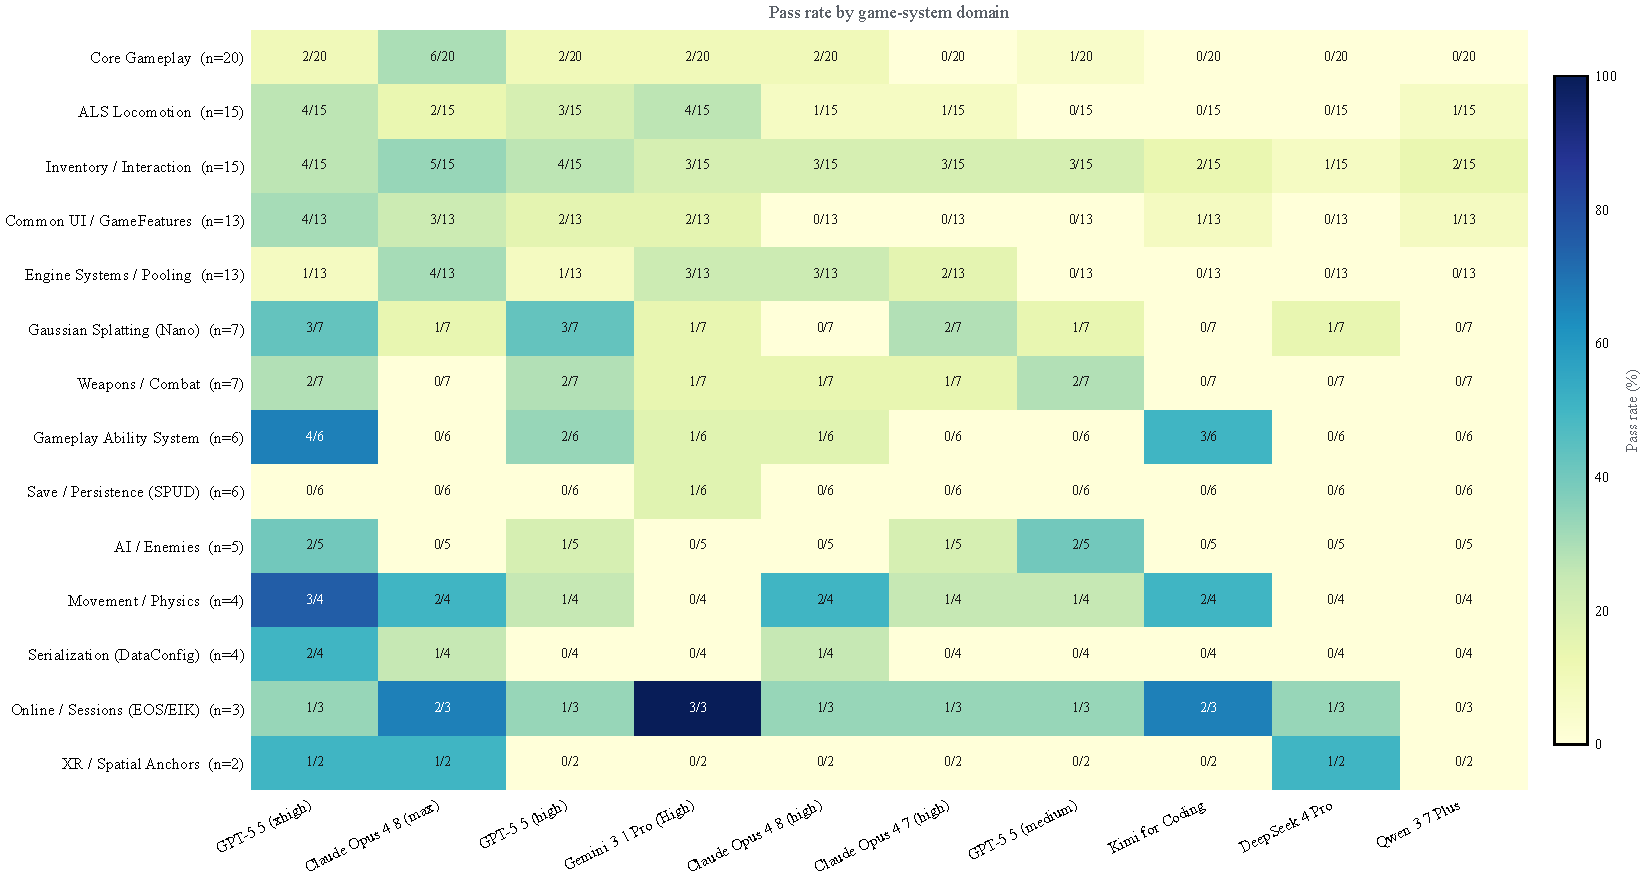
\includegraphics[width=\linewidth]{05_pass_rate_by_domain.pdf}
\end{minipage}\hfill
\begin{minipage}{0.49\textwidth}
\centering
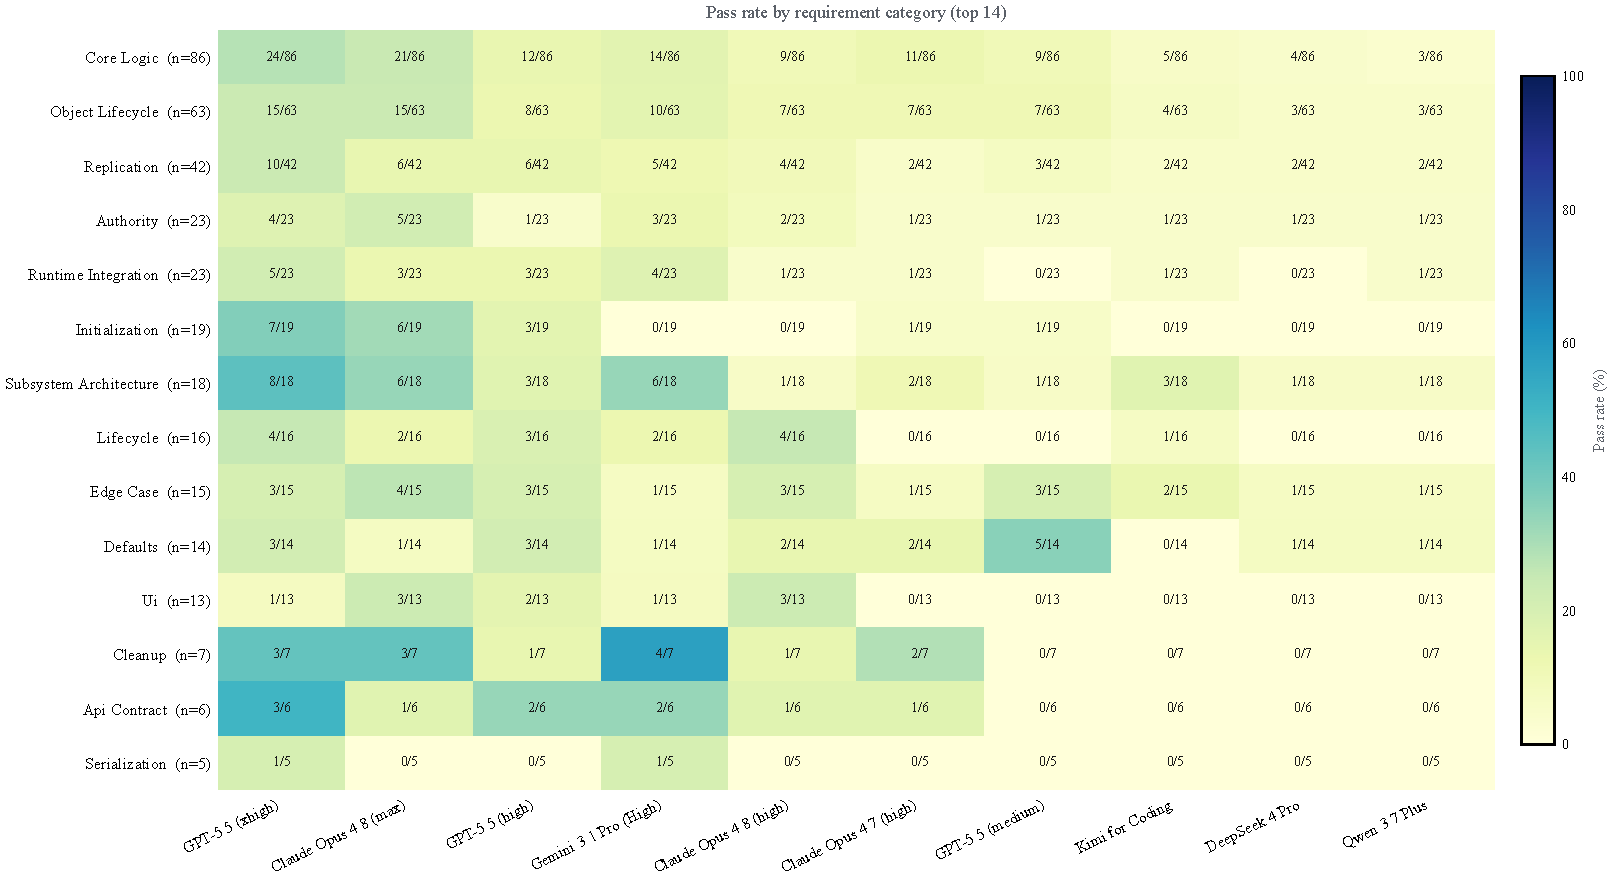
\includegraphics[width=\linewidth]{06_pass_rate_by_category.pdf}
\end{minipage}
\caption{Supplemental pass@1 breakdowns by task metadata. Left: pass@1 by game-system domain. Right: pass@1 by requirement category.}
\label{fig:appendix-domain-category}
\end{figure}

Figure~\ref{fig:appendix-domain-category} checks whether the benchmark difficulty is concentrated in particular kinds of game-engine work. Because several categories contain only a small number of tasks, these plots should be read as directional evidence rather than as precise estimates for each domain. They are most useful for seeing which areas contribute to the unsolved set and for guiding future task expansion.

\begin{figure}[t]
\centering
\begin{minipage}{0.49\textwidth}
\centering
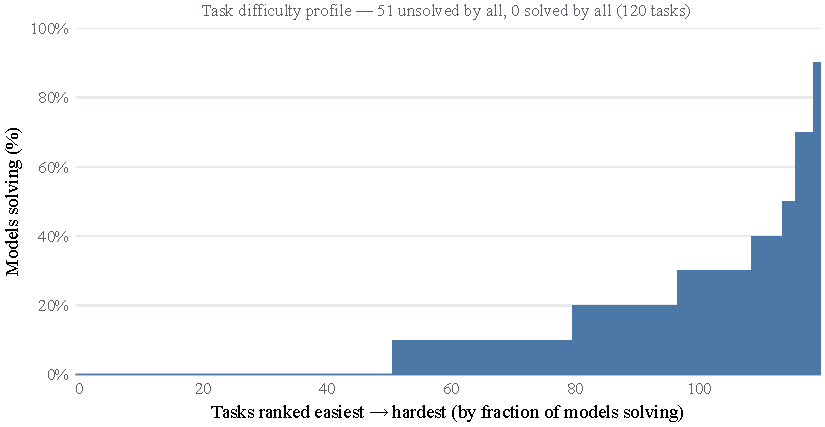
\includegraphics[width=\linewidth]{12_task_difficulty_curve.pdf}
\end{minipage}\hfill
\begin{minipage}{0.49\textwidth}
\centering
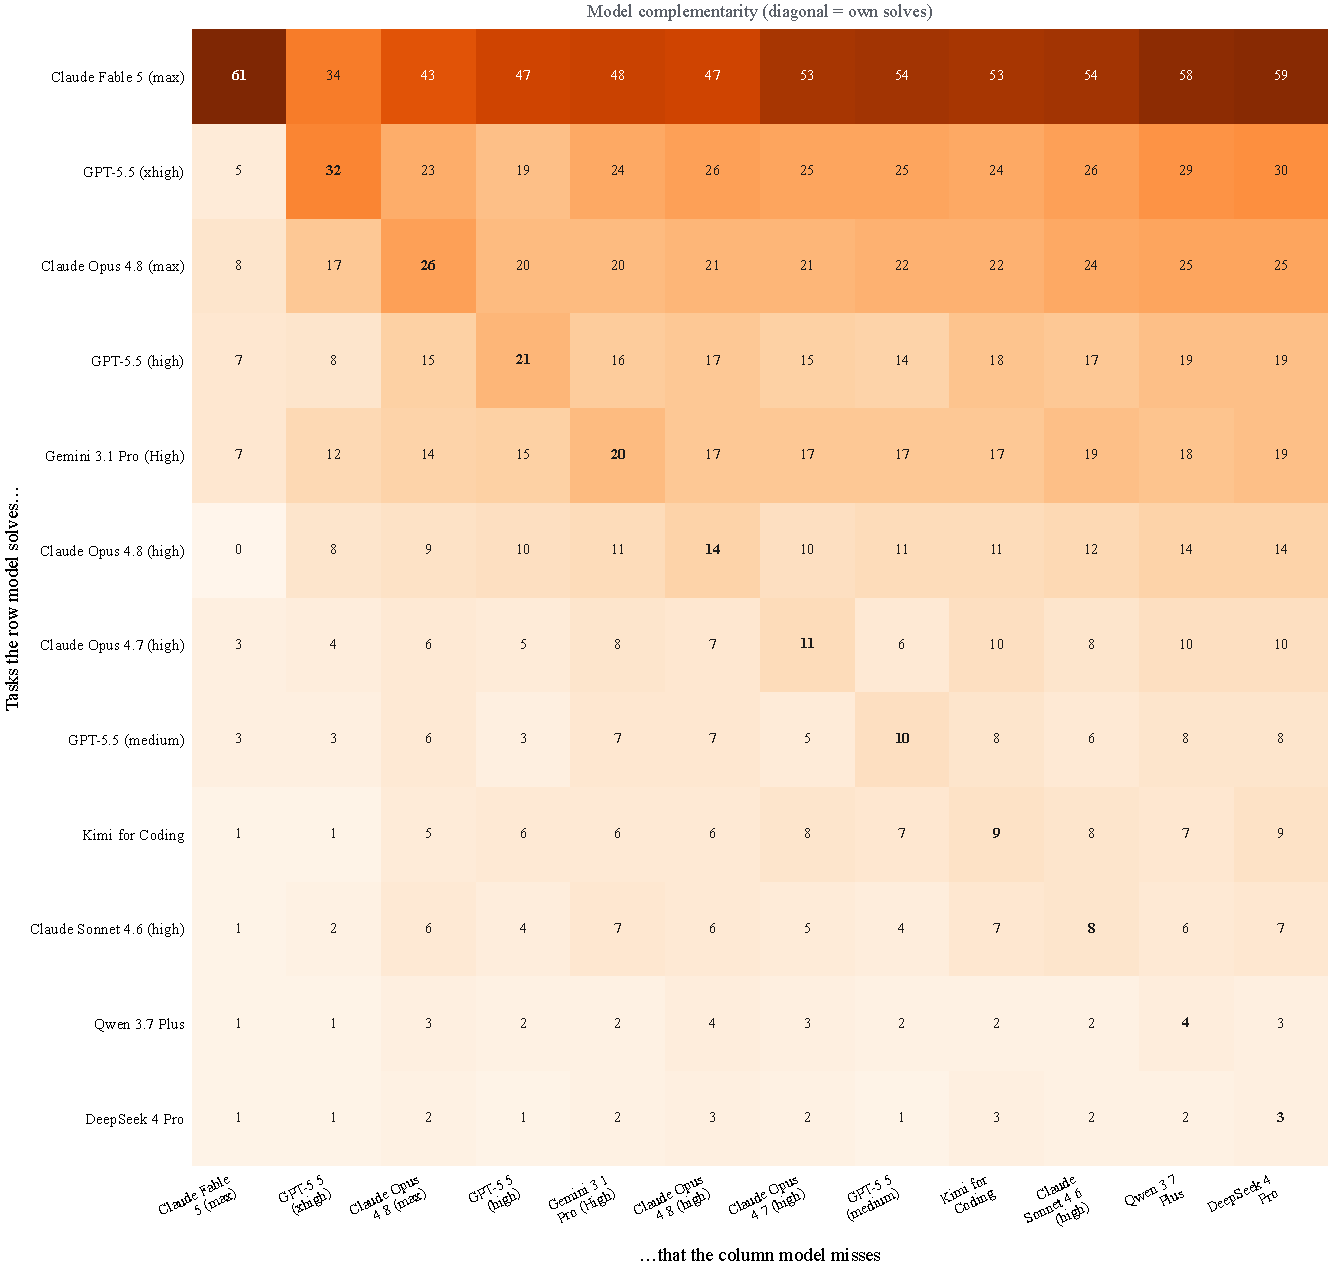
\includegraphics[width=\linewidth]{14_model_complementarity.pdf}
\end{minipage}
\caption{Supplemental task difficulty and complementarity views. Left: tasks ranked by fraction of configurations that solve them. Right: pairwise task complementarity between configurations.}
\label{fig:appendix-difficulty-complementarity}
\end{figure}

Figure~\ref{fig:appendix-difficulty-complementarity} is the denser diagnostic version of the complementarity result in Figure~\ref{fig:coverage-complementarity}. The difficulty curve shows that the benchmark contains both broadly solved tasks and a substantial no-solve region. The pairwise matrix then asks a different question: for each pair of configurations, how many tasks does one solve that the other misses? Large off-diagonal values mean that the leaderboard is not simply a nested ordering. Appendix~\ref{app:complementarity-examples} walks through two concrete task examples behind this pattern.

\begin{figure}[t]
\centering
\begin{minipage}{0.49\textwidth}
\centering
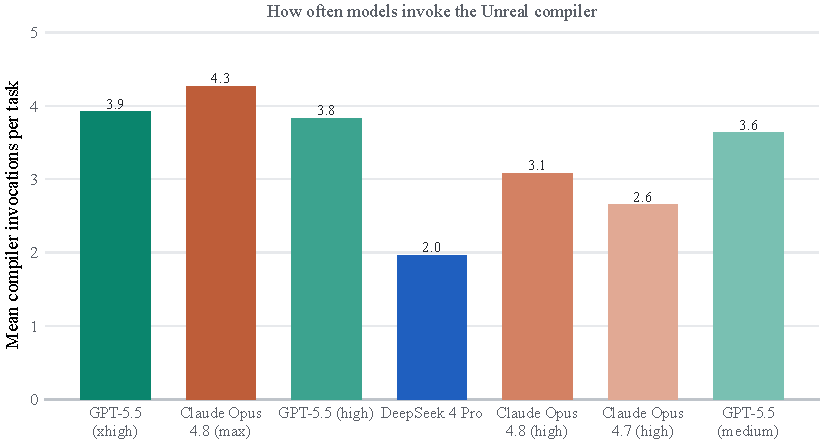
\includegraphics[width=\linewidth]{16_compile_calls.pdf}
\end{minipage}\hfill
\begin{minipage}{0.49\textwidth}
\centering
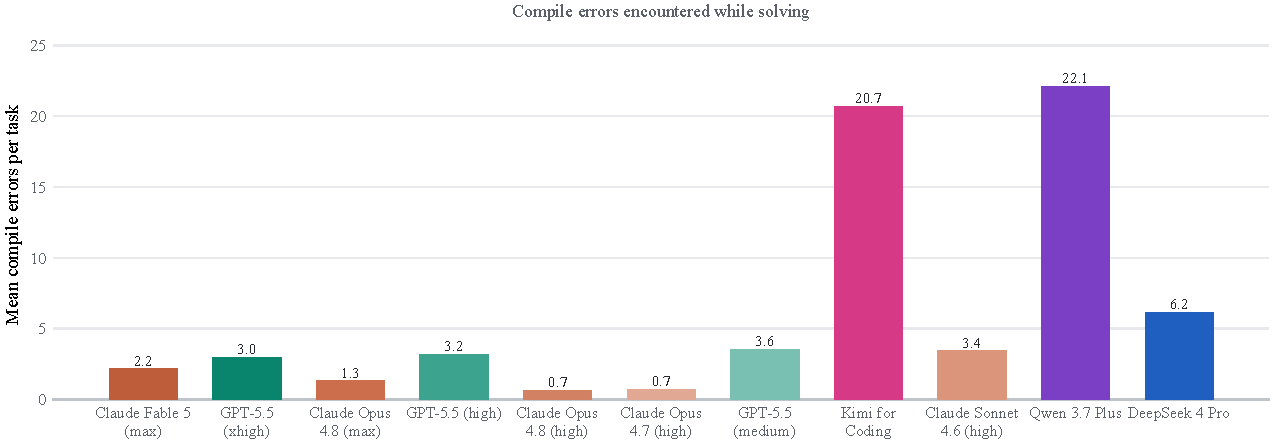
\includegraphics[width=\linewidth]{17_compile_errors.pdf}
\end{minipage}
\caption{Supplemental compile diagnostics from available trajectories. Left: mean number of Unreal compiler invocations per task. Right: mean number of compile errors encountered during solving.}
\label{fig:appendix-compile-diagnostics}
\end{figure}

Figure~\ref{fig:appendix-compile-diagnostics} summarizes compiler use when the wrapper trajectory exposes it. The figure should be interpreted as a wrapper-visible behavior diagnostic, not as a complete comparison for every agent interface. It helps separate configurations that actively iterate through Unreal compilation from configurations where compile behavior is either less frequent or less visible in the saved trace.

\begin{figure}[t]
\centering
\begin{minipage}{0.49\textwidth}
\centering
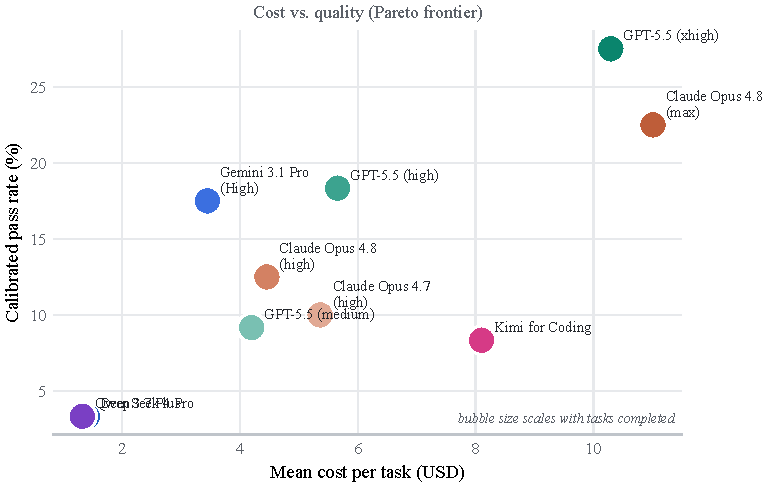
\includegraphics[width=\linewidth]{08_cost_vs_pass_rate.pdf}
\end{minipage}\hfill
\begin{minipage}{0.49\textwidth}
\centering
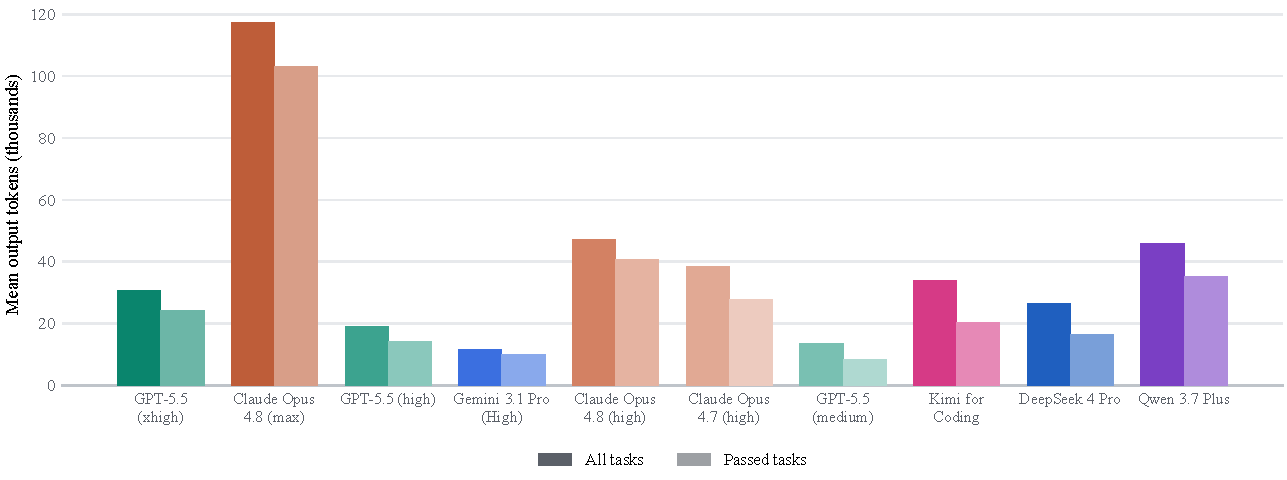
\includegraphics[width=\linewidth]{09_output_tokens.pdf}
\end{minipage}
\caption{Supplemental resource-use diagnostics. Left: cost versus task-pass rate where cost data is available. Right: output tokens per task.}
\label{fig:appendix-resource-diagnostics}
\end{figure}

Figure~\ref{fig:appendix-resource-diagnostics} provides the resource context for the efficiency discussion in the main text. Cost and token accounting are not equally complete for every wrapper, so these plots are best treated as available-data diagnostics rather than as a definitive pricing comparison. They still show that higher pass@1 is not free: stronger configurations often spend more inference, compilation, or review budget per task.

\FloatBarrier
\section{Complementarity Examples}
\label{app:complementarity-examples}
Figure~\ref{fig:coverage-complementarity} and Figure~\ref{fig:appendix-difficulty-complementarity} show that model capability is not fully nested. This matters because a pure leaderboard view would suggest that a lower-ranked model adds little once a stronger model is available. The task-level matrix shows a different picture: some tasks are recovered by one configuration while being missed by configurations that are stronger overall. Complementarity therefore indicates that the benchmark is testing multiple kinds of game-engine reasoning rather than one scalar notion of C++ skill.

Task \texttt{15} (AI Controller + Behavior Tree) is solved only by \texttt{GPT-5.5} at \texttt{xhigh} in the active 110-task matrix. The task requires the agent to start an assigned behavior tree, register a blackboard observer after blackboard initialization, notify a player through a client RPC when the target changes, set team affiliation before pawn component registration, implement EQS target context lookup, and fill several behavior-tree services, tasks, and decorators. This is not a large rendering or UI task; it is an AI-control and initialization-order task where correctness depends on several behavior-tree and perception pieces becoming available at the right time. Its one-model success shows that \texttt{GPT-5.5} recovers at least some AI orchestration behavior that the other configurations miss.

Task \texttt{19} (Generated Map Orchestrator) shows the opposite direction. It is solved only by \texttt{claude-fable-5} at \texttt{max}. The task asks the model to populate a procedural grid at round start, run expensive cell assignment off the game thread, reuse pooled actors across regenerations, replicate generated-map containers and generation tokens, fire exactly one ready signal after local actors are present, and handle runtime map-size changes. This task combines replication, object lifecycle, pooling, asynchronous generation, and readiness signaling. Its one-model success shows why complementarity is useful: even the strongest non-Fable configurations miss some cross-system lifecycle and replication problems that another model can solve.

These examples make the off-diagonal entries in the complementarity matrix concrete. They are not just statistical noise around the pass@1 ranking. They correspond to qualitatively different task structures: behavior-tree initialization and AI control in one case, procedural map generation with pooling and replicated readiness in the other. For benchmark design, this means that additional model runs can reveal distinct capability pockets, while the no-solve tasks still identify behaviors that likely require better training, tooling, or task-specific reasoning.

\section{Reproducibility Notes}
The current repository already contains the key scripts required to reproduce benchmark runs, including
\path{GameEngineBench/src/ue_benchmark_runner.py} and
\path{GameEngineBench/src/authoring/generate_task_tests.py}.
The task packages live under \path{tasks_unreal/<task-id>/}, and saved benchmark snapshots live under
\path{tasks_unreal/test_result/}.
The main text reports the execution setup used for the evaluated task set; a stronger public release should bundle explicit OS, hardware, wrapper-version, and prompt-metadata files alongside the benchmark artifacts.

\end{document}
